% moved to abstract
%The system must autonomously scan for, identify, and track discrete targets. Once a target is identified, the turret must center itself on target and, if the turret has a reasonable chance to hit the target, fire. The system must be able to distinguish between valid targets and those that should not be fired upon, and operate accordingly..


\subsection{Existing designs}

 
We turned to instructables to find existing examples of turret designs to compare their features to our constraints. Instructables hosts DIY projects from people around the world, giving good documentation on how different projects operate, and what materials they consist of, serving as an excellent source to compare all aspects of designs.
\subsubsection{Instructables Autonomous Sentry Turret}
This turret\footnote{\url{https://www.instructables.com/id/Autonomous-Sentry-Turret/}}(Figure 1) design uses a laser range finder and infrared motion sensor to determine targets. The turret sweeps a range of 100 degrees with 10 degree intervals, storing range data. Once data is recorded for the entire sweep and stored data, the turret starts sweeping the same range, and if the range is different from the stored value, the turret fires a third of its clip down the bearing. The turret then waits for the moment sensor to be tripped to begin sweeping again.


The greatest issue this turret has with our problem statement is a lack of discrimination. A difference in rangefinder data will trigger the turret, for example, a door that was either opened or closed mid sweep would be treated as a target. Also, if a person were to walk by the turret during its initial sweep, when the ranges are being determined, the turret would, on its second sweep register a target and begin firing. Furthermore, once the turret starts to fire, the bearing is static, so many shots would be wasted on a moving target. If instead a change in range was coupled with the IR sensor, the system could avoid some false positives.
\begin{figure}[ht]
    \centering
    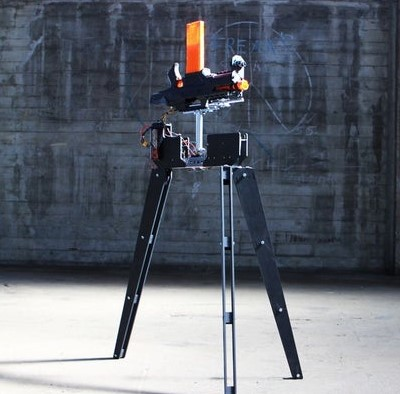
\includegraphics[scale=.4]{autosentTurret.jpg}
    \caption{Autonomous Sentry Turret}
    \label{fig:first turret}
\end{figure}



\subsubsection{Instructables Face Tracking Pan-Tilt Camera}
This\footnote{\url{https://www.instructables.com/id/Face-Tracking-Pan-Tilt-Camera/}} (Figure 2)is a gimbal system for a camera meant to track faces (or other objects depending on training). The system must be provided with several photos of whatever image it is meant to detect. The system uses machine learning to determine what constitutes a face (or target of choice), then gives the coordinates of the target relative to the camera’s center. This data is then used to center the servo, using a proportional control.
        
The low point of this solution seems to be the control algorithm. The demonstration videos show slow and imperfect response (with a large steady state error). Furthermore, the system in this project is only built to be able to detect one type of target at a time. It can only positively identify one type of target, and cannot determine between different types of targets. Furthermore, having more than one target in frame could cause the system to oscillate between the two.
\begin{figure}[h!]
    \centering
    \includegraphics[scale=.4]{facepalmtracking.jpg}
    \caption{Face Tracking}
    \label{fig:face palm}
\end{figure}


\subsubsection{Instructables Portal Turret}
This\footnote{\url{https://www.instructables.com/id/Building-a-moving-and-tracking-Portal-Turret/}}(Figure 3) is a 3D printed turret system that can be operated in two modes autonomously or by joystick controlled. When connected to a computer it uses software to detect and track a target designated target. It does this by constantly taking a stream of data and converting it to motor movement. The turret is smart enough to recognize when the target is moving and when the target moves out of the view of the camera.  The software that runs this turret is highly similar to the one that we will use in our own project except it is written in Arduino. 

The biggest weakness of the design however is that it requires the use of a 3D printer to make the pieces with enough precision that the guns, motors, and  electrical work can all fit within the shell. Another issue with this design for our project is it would require us to learn a new language to code the turret.  
\begin{figure}[h!]
    \centering
    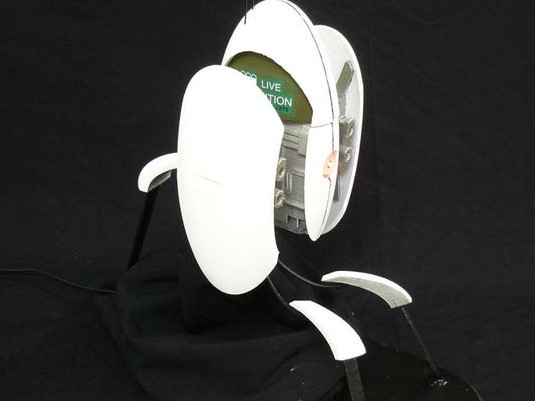
\includegraphics[scale=.3]{turret design2.jpg}
    \caption{Portable Turret}
    \label{fig:portable turret}
\end{figure}

\subsubsection{Instructables Robotic Talking Turret}
This turret design\footnote{\url{https://www.instructables.com/id/Robotic-Talking-Turret/}}(Figure 4) uses a rangefinder along with the Stampy method to track targets. The rangefinder is constantly sweeping back and forth until it finds a target. Once the target is found the turret starts sweeping and firing. The design of the turret also allows it to know when it is being picked up or tipped over. Both of these actions would stop the rangefinder from moving. 
The largest issues in this design is that it will track and fire at an object whether it be a target or not as long as it is within the set range of the range finder. Meaning that if someone where to walk past or another object be within the set range the turret would track it and fire. Another large issue that this design has is that it fires as soon as an object is within range no matter where the turret is a lined.
\begin{figure}[h!]
    \centering
    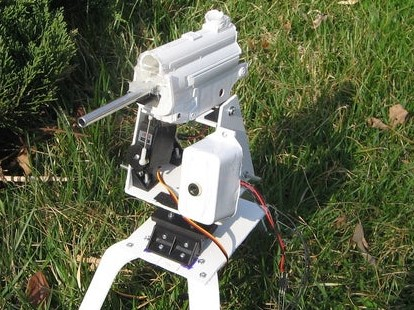
\includegraphics[scale=.4]{turret design 3.jpg}
    \caption{Robotic Talking Turret}
    \label{fig:talking turret}
\end{figure}
% instructor comment: Probably need something here like a table or chart comparing the designs with yours alongside
